\section{Interferometer Design and Hardware Configuration}

\begin{figure}[htbp]
    \centering
    \begin{subfigure}{0.45\textwidth}
        \centering
        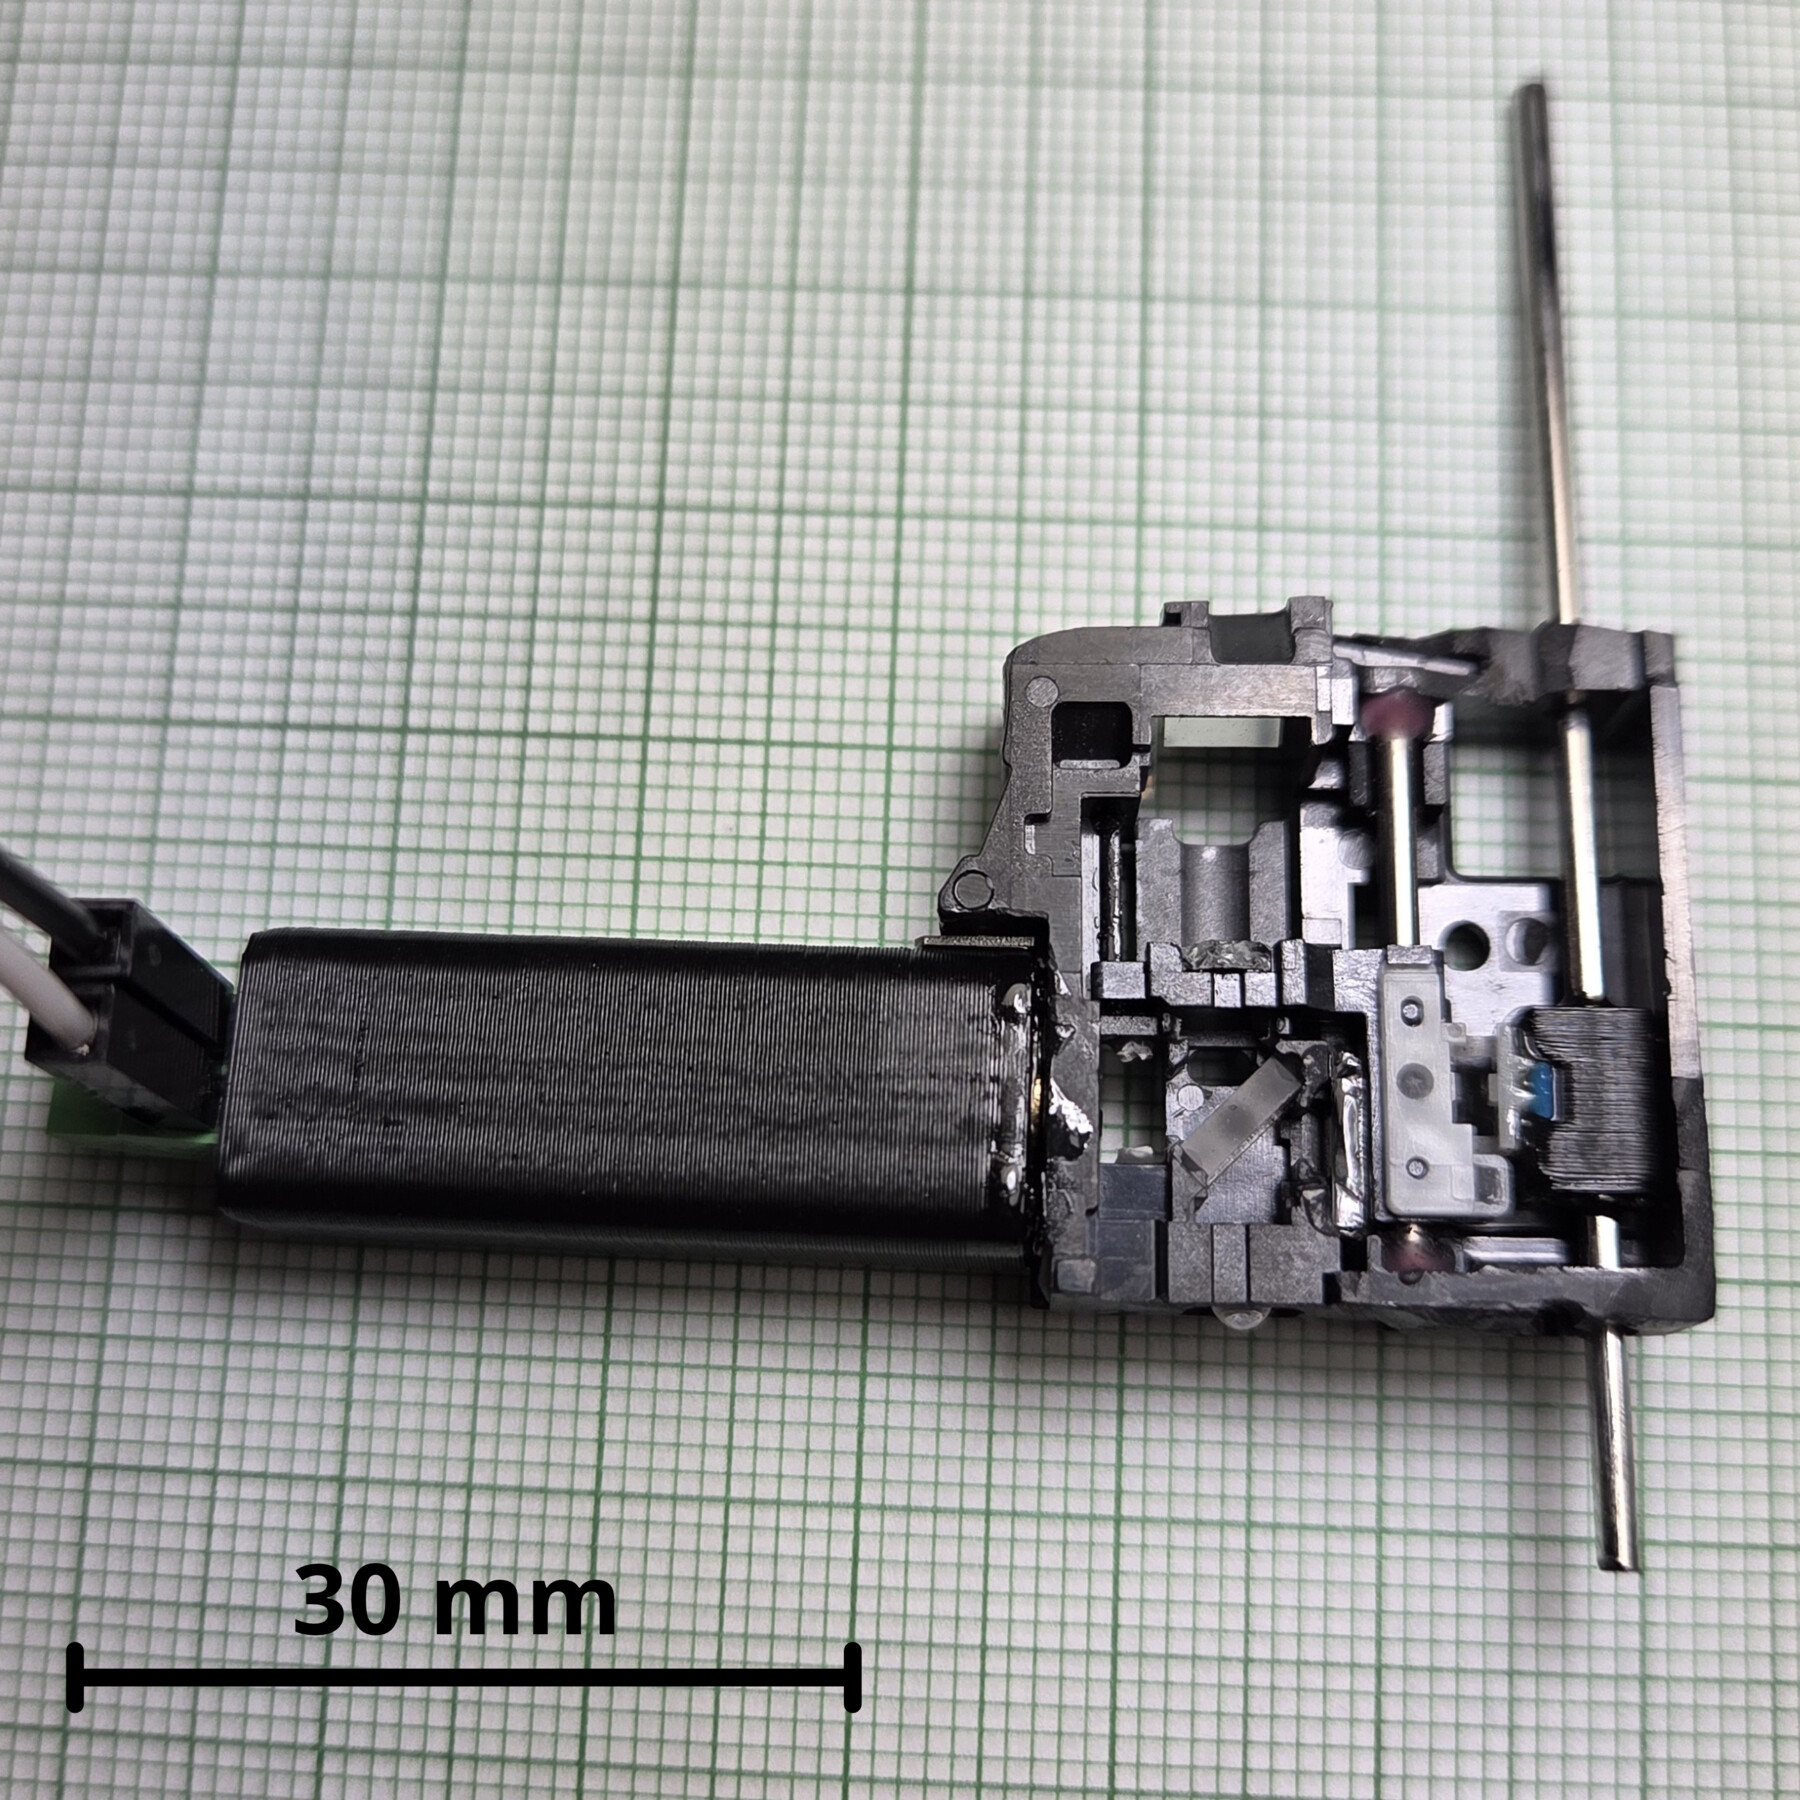
\includegraphics[width=\textwidth]{images/interferometer_top_big_compressed.jpg}
        \caption{Interferometer}
        \label{fig:interferometer_top}
    \end{subfigure}\hfill
    \begin{subfigure}{0.45\textwidth}
        \centering
        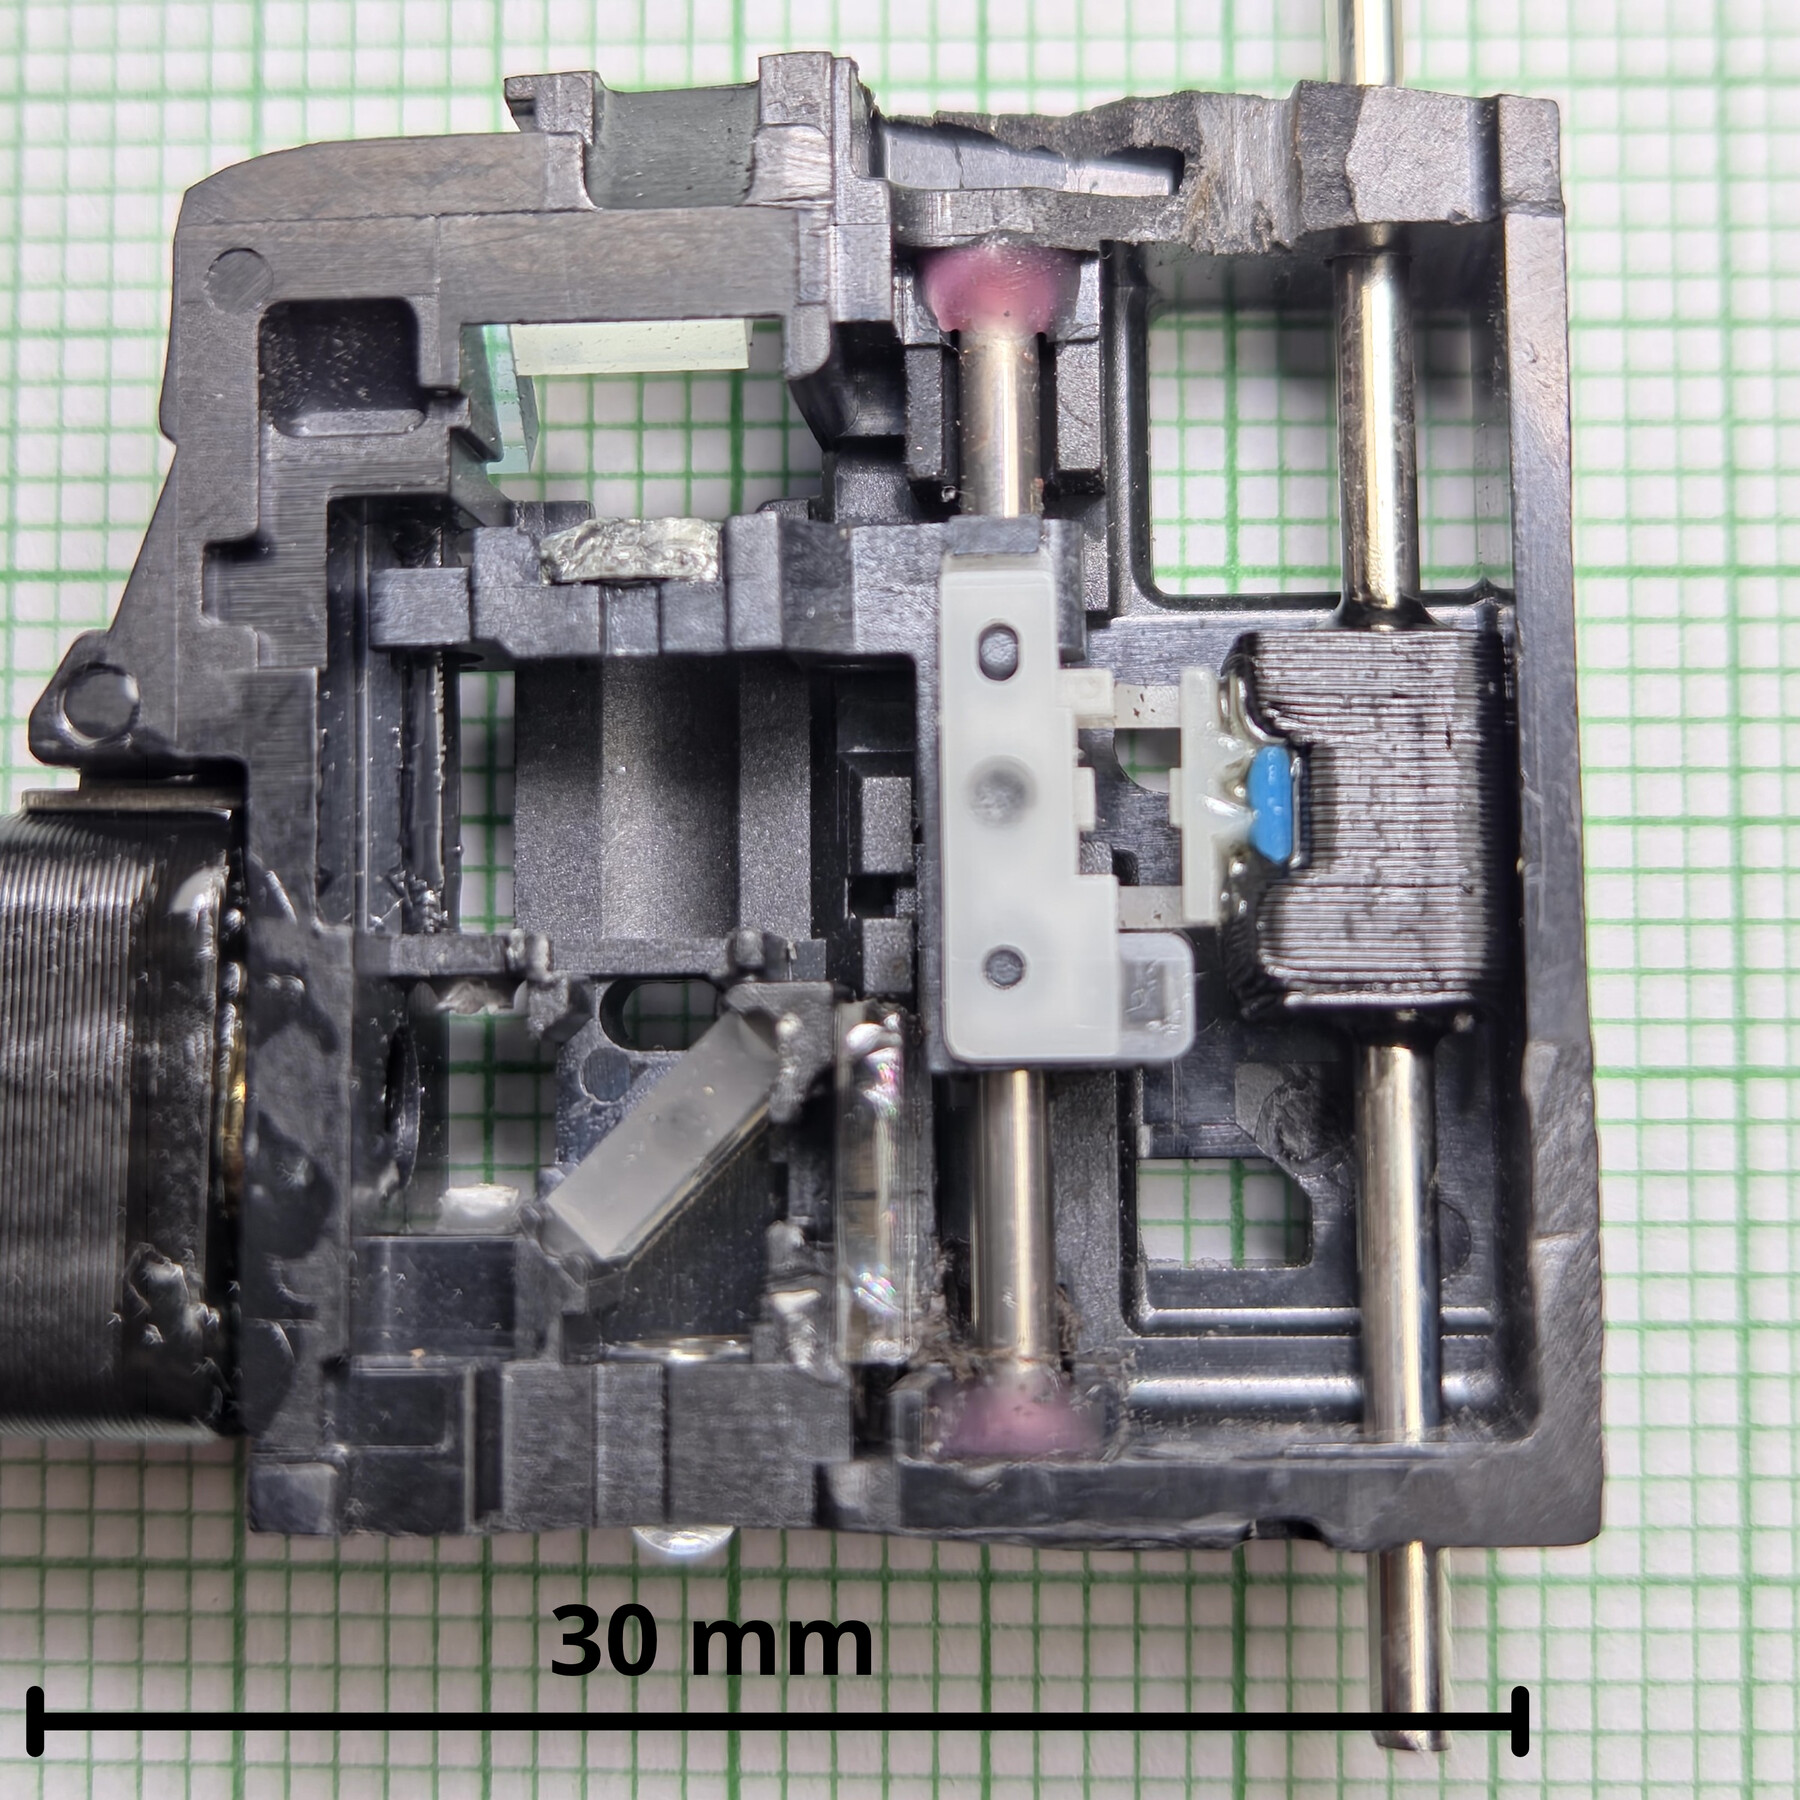
\includegraphics[width=\textwidth]{images/interferometer_top_zoomed_test.jpg}
        \caption{Interferometer (Zoomed)}
        \label{fig:interferometer_top_zoomed}
    \end{subfigure}
    \caption{Interferometer Experimental Setup. a) Top view; b) Zoomed top view with details of the mirrors and axis mounting.}
    \label{fig:interferometer_setup}
\end{figure}


In the \cref{fig:interferometer_setup} we can see the top view of the  interferometer constructed as shown in the figure, the interferometer is compact and robust, with a design that minimizes vibrations and misalignments by using a rigid casing and keeping the optical components close together, this creates a stable optical path and reduces the impact of external disturbances due to the vibrations of the system as a whole. The compactness of the device also allows for easier alignment of the optical components, as the distances between them are small, reducing the chances of misalignment when the shafts transfer the actuator motion into the movable mirror, the thermal expansion effects are also reduced due to uniform heat conduction between the components because of their proximity, improving the overall performance of the interferometer. The design compactness also allows for easy coupling to other systems and can be integrated into larger experimental setups without taking up much space, making it suitable for applications where space is limited.

\begin{figure}[htbp]
    \centering
    \begin{subfigure}{0.45\textwidth}
        \centering
        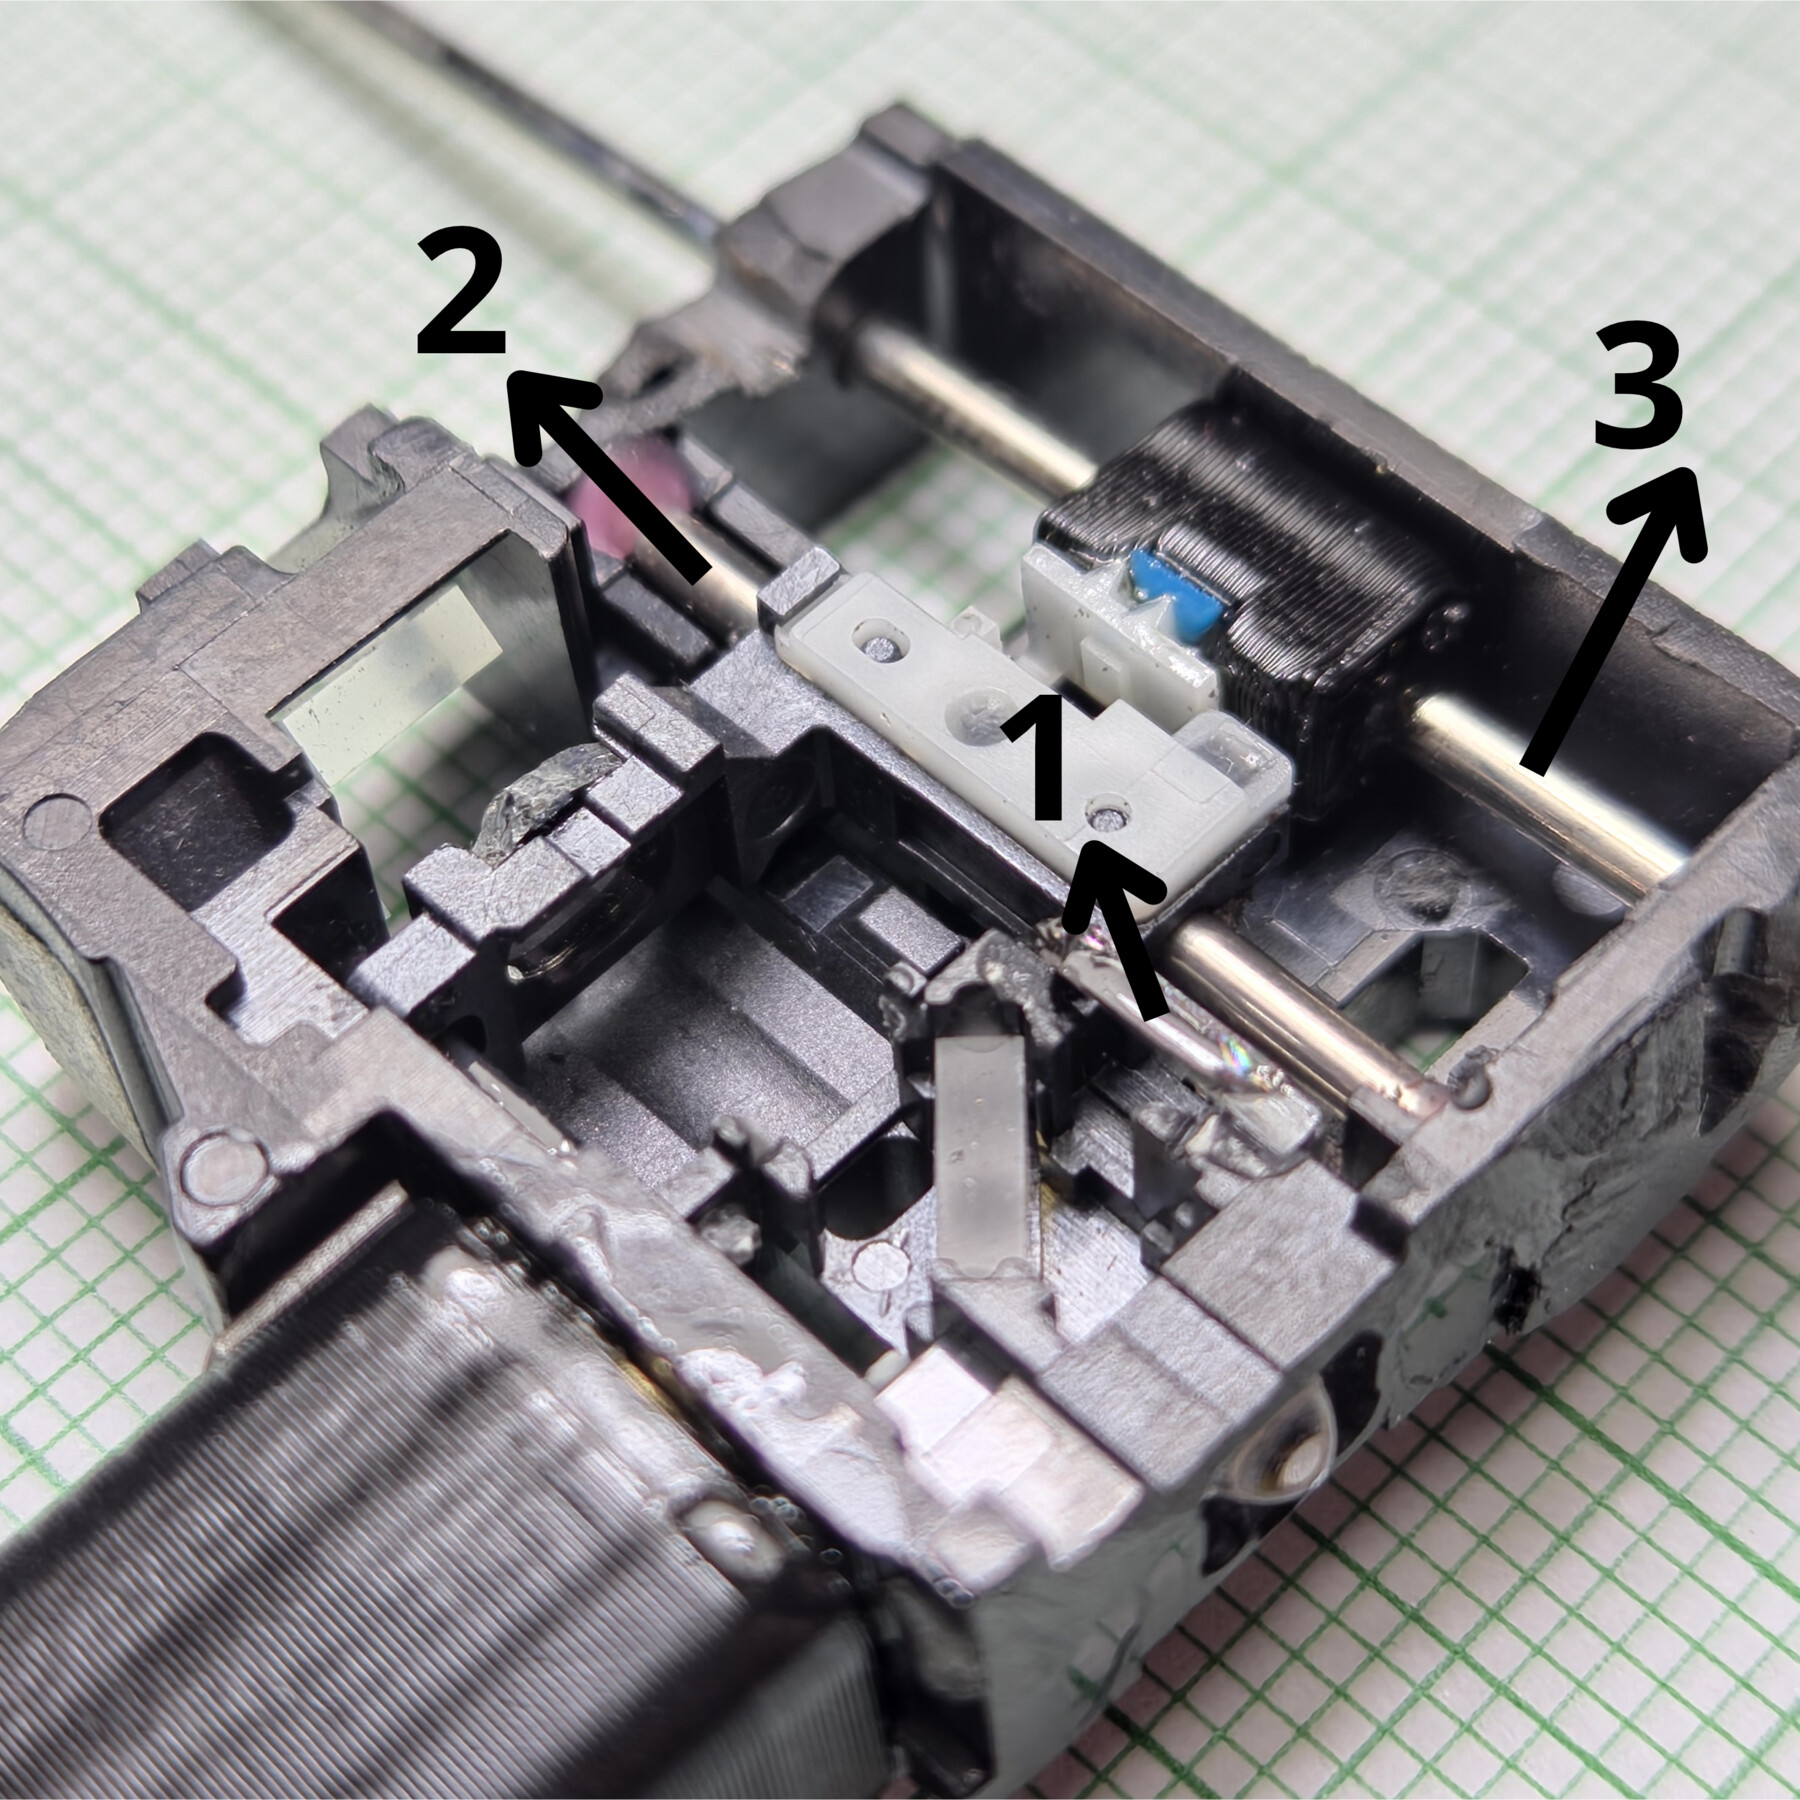
\includegraphics[width=\textwidth]{images/interferometer_side_compressed.jpg}
        \caption{Interferometer side view}
        \label{fig:interferometer_side_a}
    \end{subfigure}\hfill
    \begin{subfigure}{0.45\textwidth}
        \centering
        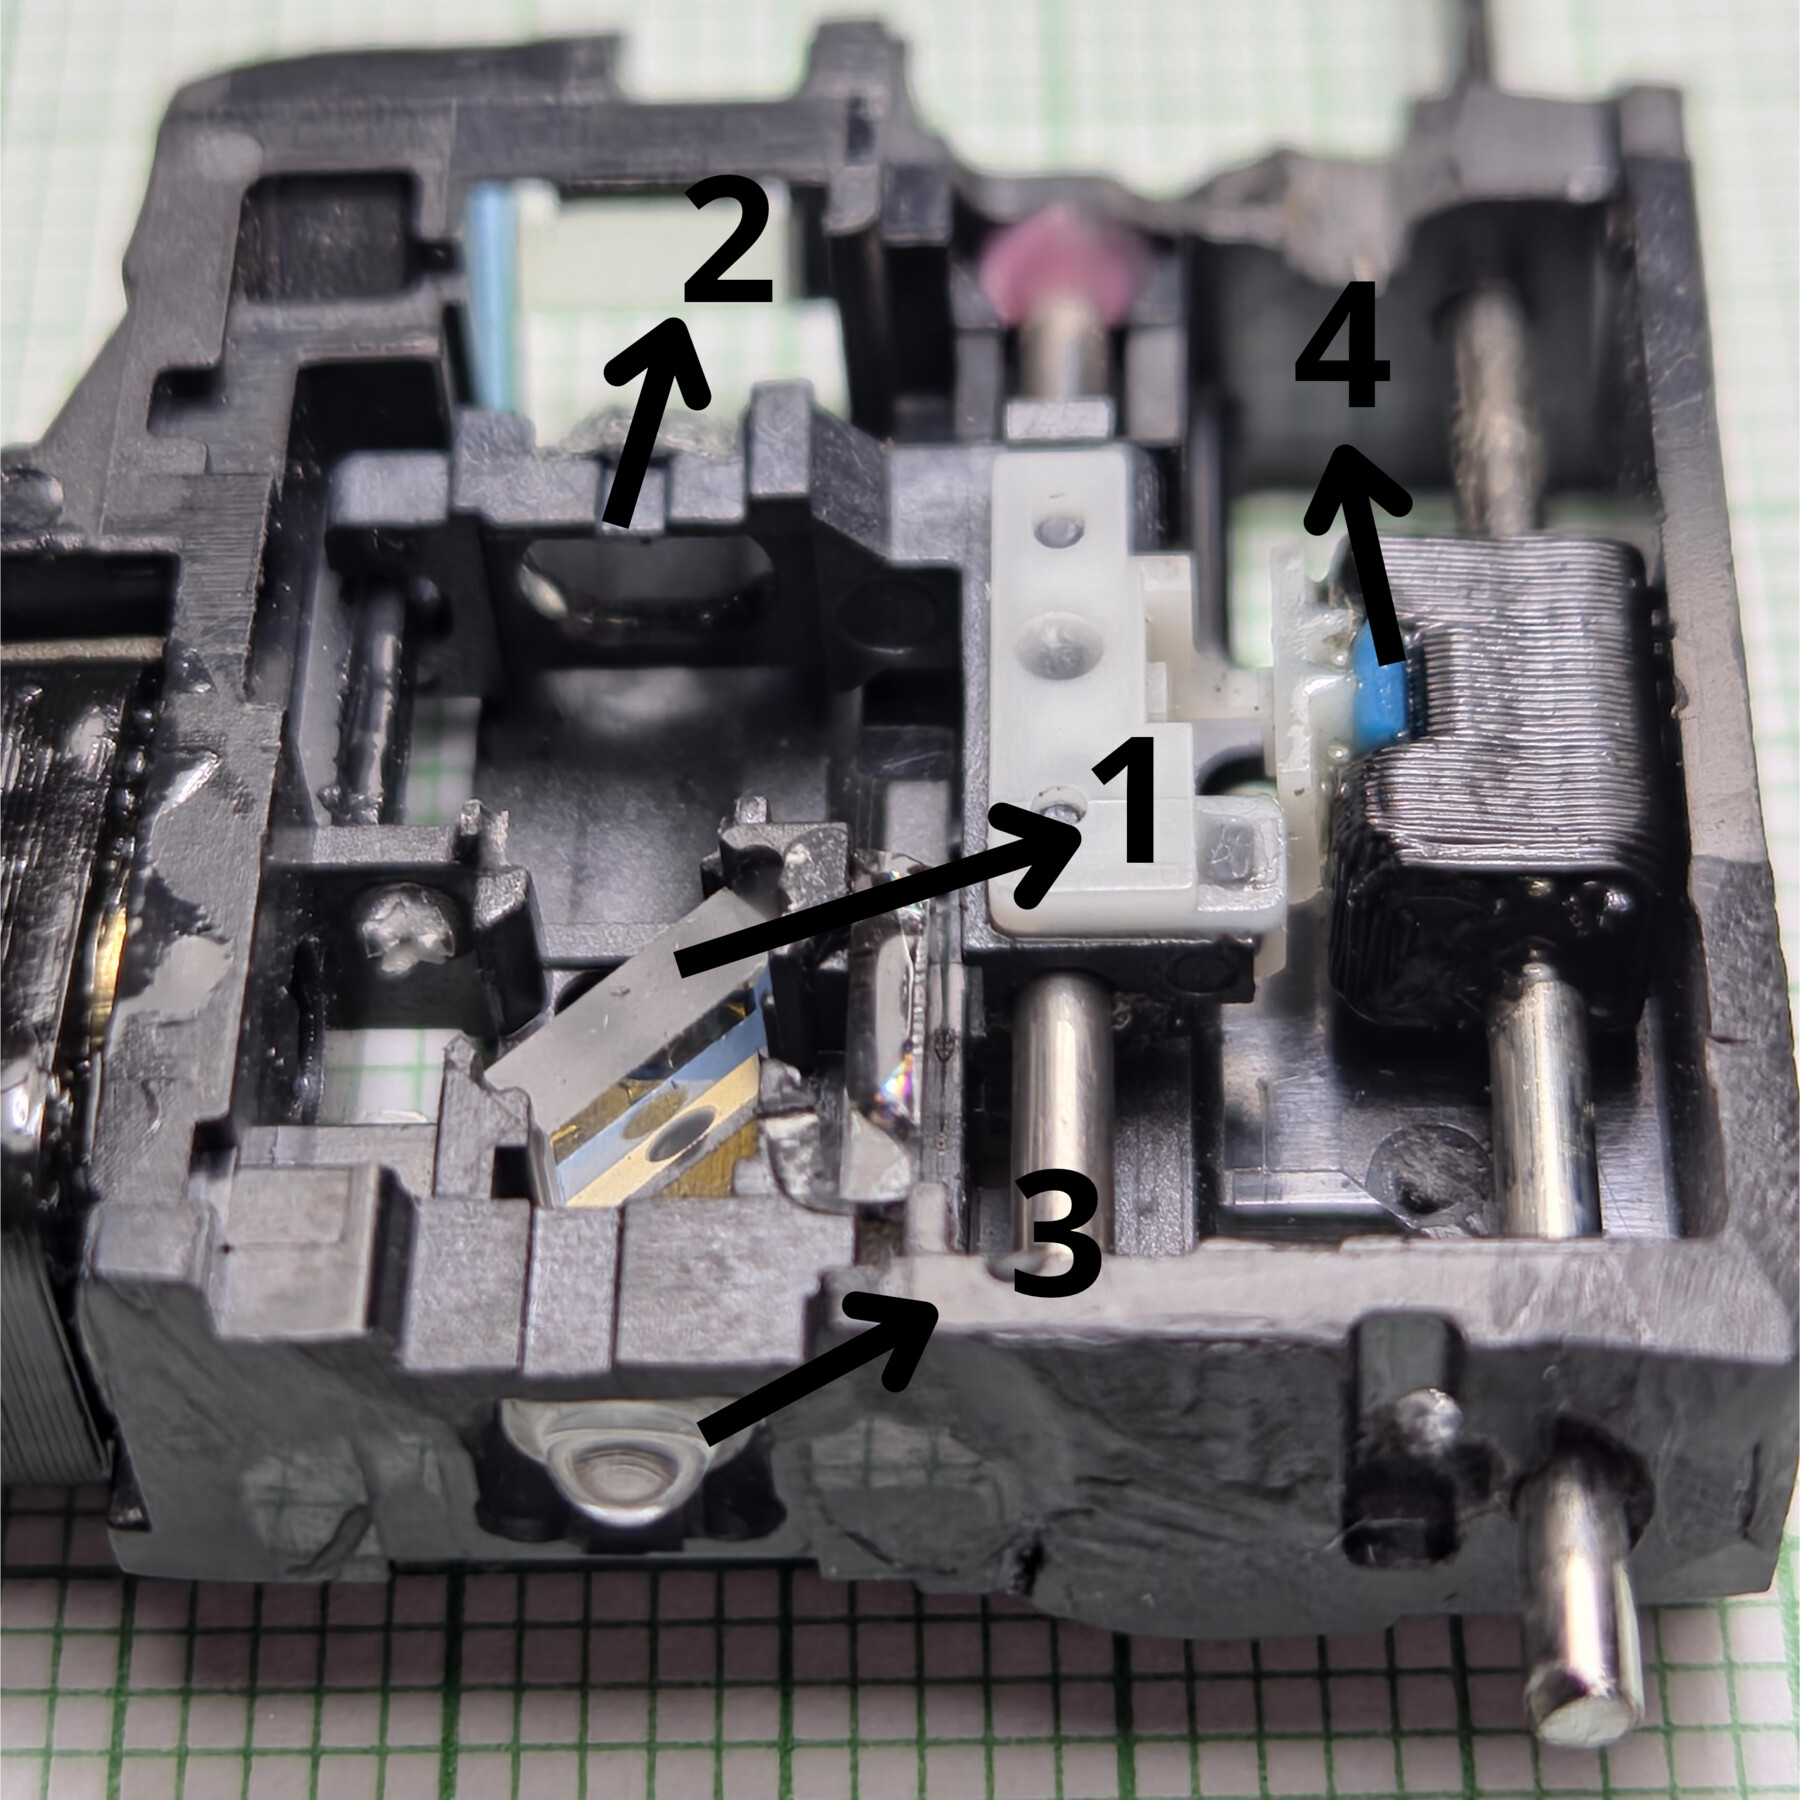
\includegraphics[width=\textwidth]{images/interferometer_side_front_compressed.jpg}
        \caption{Interferometer front view}
        \label{fig:interferometer_side_front_b}
    \end{subfigure}
    \caption{Interferometer Experimental Setup. a) Side view, 1: Fixed mirror, 2: Movable mirror shaft, 3: Movable needle shaft (transfering the motion the the outside of the interferometer casing); b) Front view, 1: Beam splitter, 2: Movable mirror, 3: Divergent lens, 4: Junction between the two shafts.}
    \label{fig:interferometer_sides}
\end{figure}

The experimental setup contains a compact Michelson interferometer integrated directly into a recycled optical unit from a Blu-ray player, as detailed in \cref{fig:interferometer_sides}. A critical mechanical feature of this implementation is the decoupling and motion-transfer assembly. The movable mirror is mounted on a precision sliding shaft (labeled 2 in \cref{fig:interferometer_side_a}) that runs parallel to a secondary movable needle shaft (labeled 3 in \cref{fig:interferometer_side_a}). These two shafts are mechanically linked via a small compliant flexure junction (labeled 4 in \cref{fig:interferometer_side_front_b}). This flexure is crucial for isolating the movable mirror from external mechanical disturbances; it acts as a vibration-damping filter that prevents high-frequency mechanical noise or binding forces from the outside actuation mechanism from distorting the mirror displacement. The needle shaft extends outward through the interferometer casing to interface with the external actuation system being characterized.

To maintain optical integrity during assembly, all internal optical components—including the beamsplitter, fixed mirror, movable mirror, and divergent lens (labeled 3 in \cref{fig:interferometer_side_front_b}) were secured using UV-curable resin. This bonding method was specifically chosen over traditional solvent-based glues to prevent out-gassing and volatile residue condensation on the delicate optical surfaces.

\subsection{Pattern Obtained}
\label{sec:pattern_obtained}

\begin{figure}[htbp]
    \centering
    \begin{subfigure}{0.45\textwidth}
        \centering
        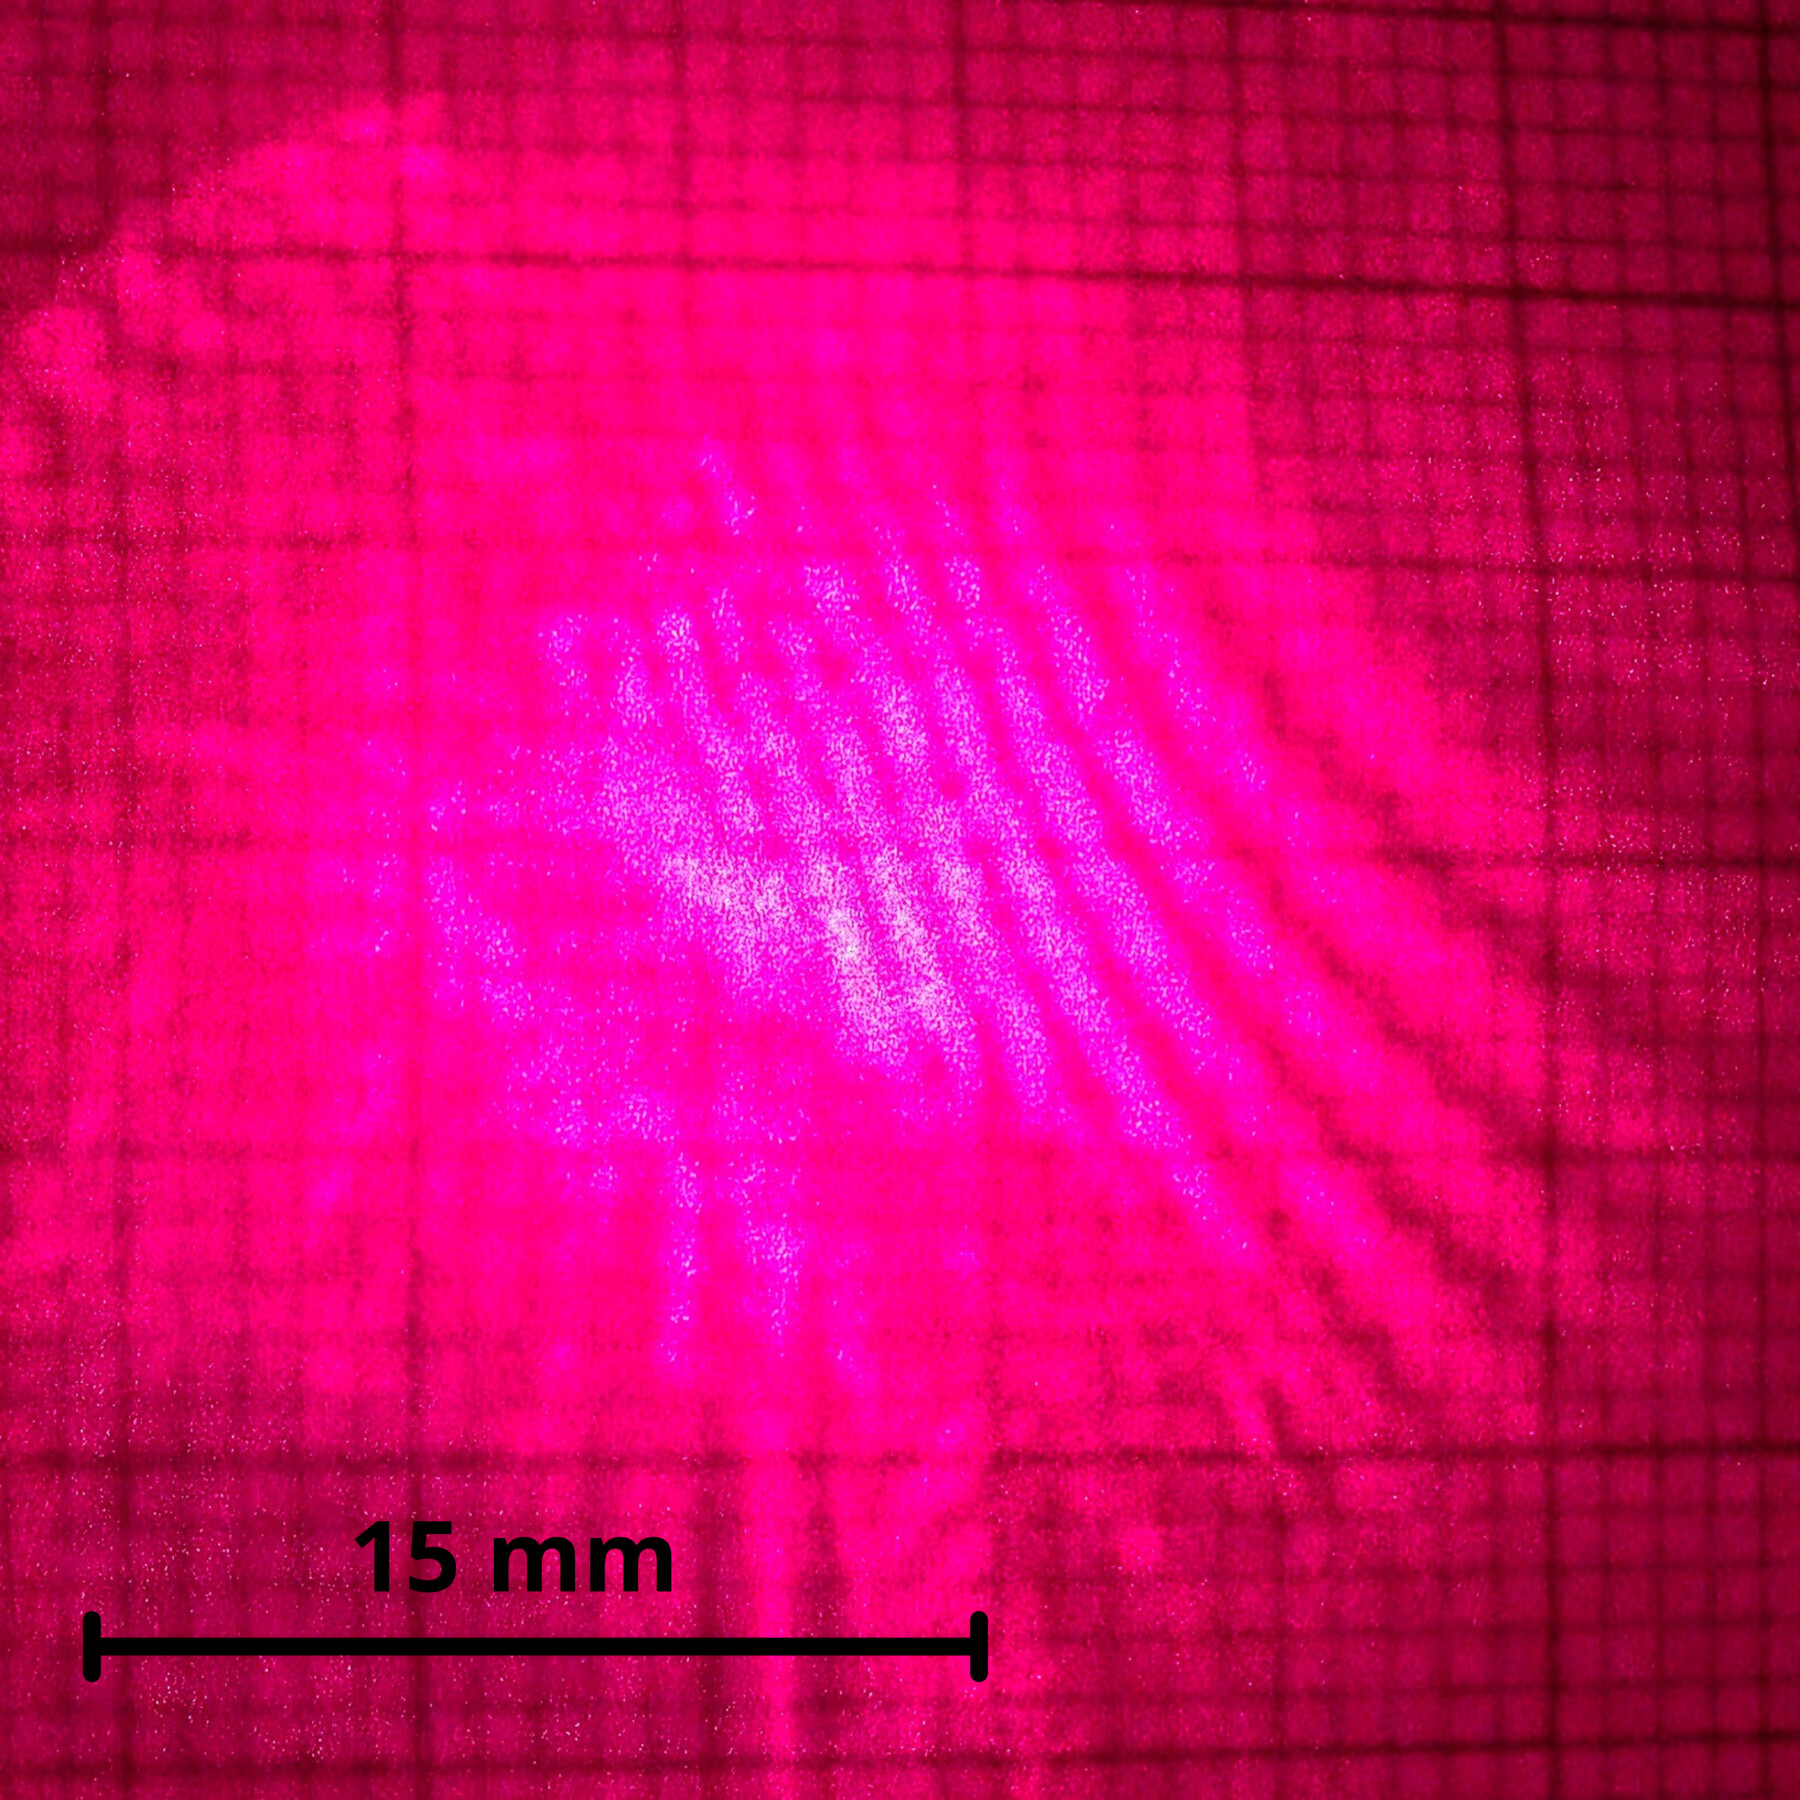
\includegraphics[width=\textwidth]{images/pattern_2mm_back_compressed.jpg}
        \caption{Pattern 2mm}
        \label{fig:pattern_2mm_back_a}
    \end{subfigure}\hfill
    \begin{subfigure}{0.45\textwidth}
        \centering
        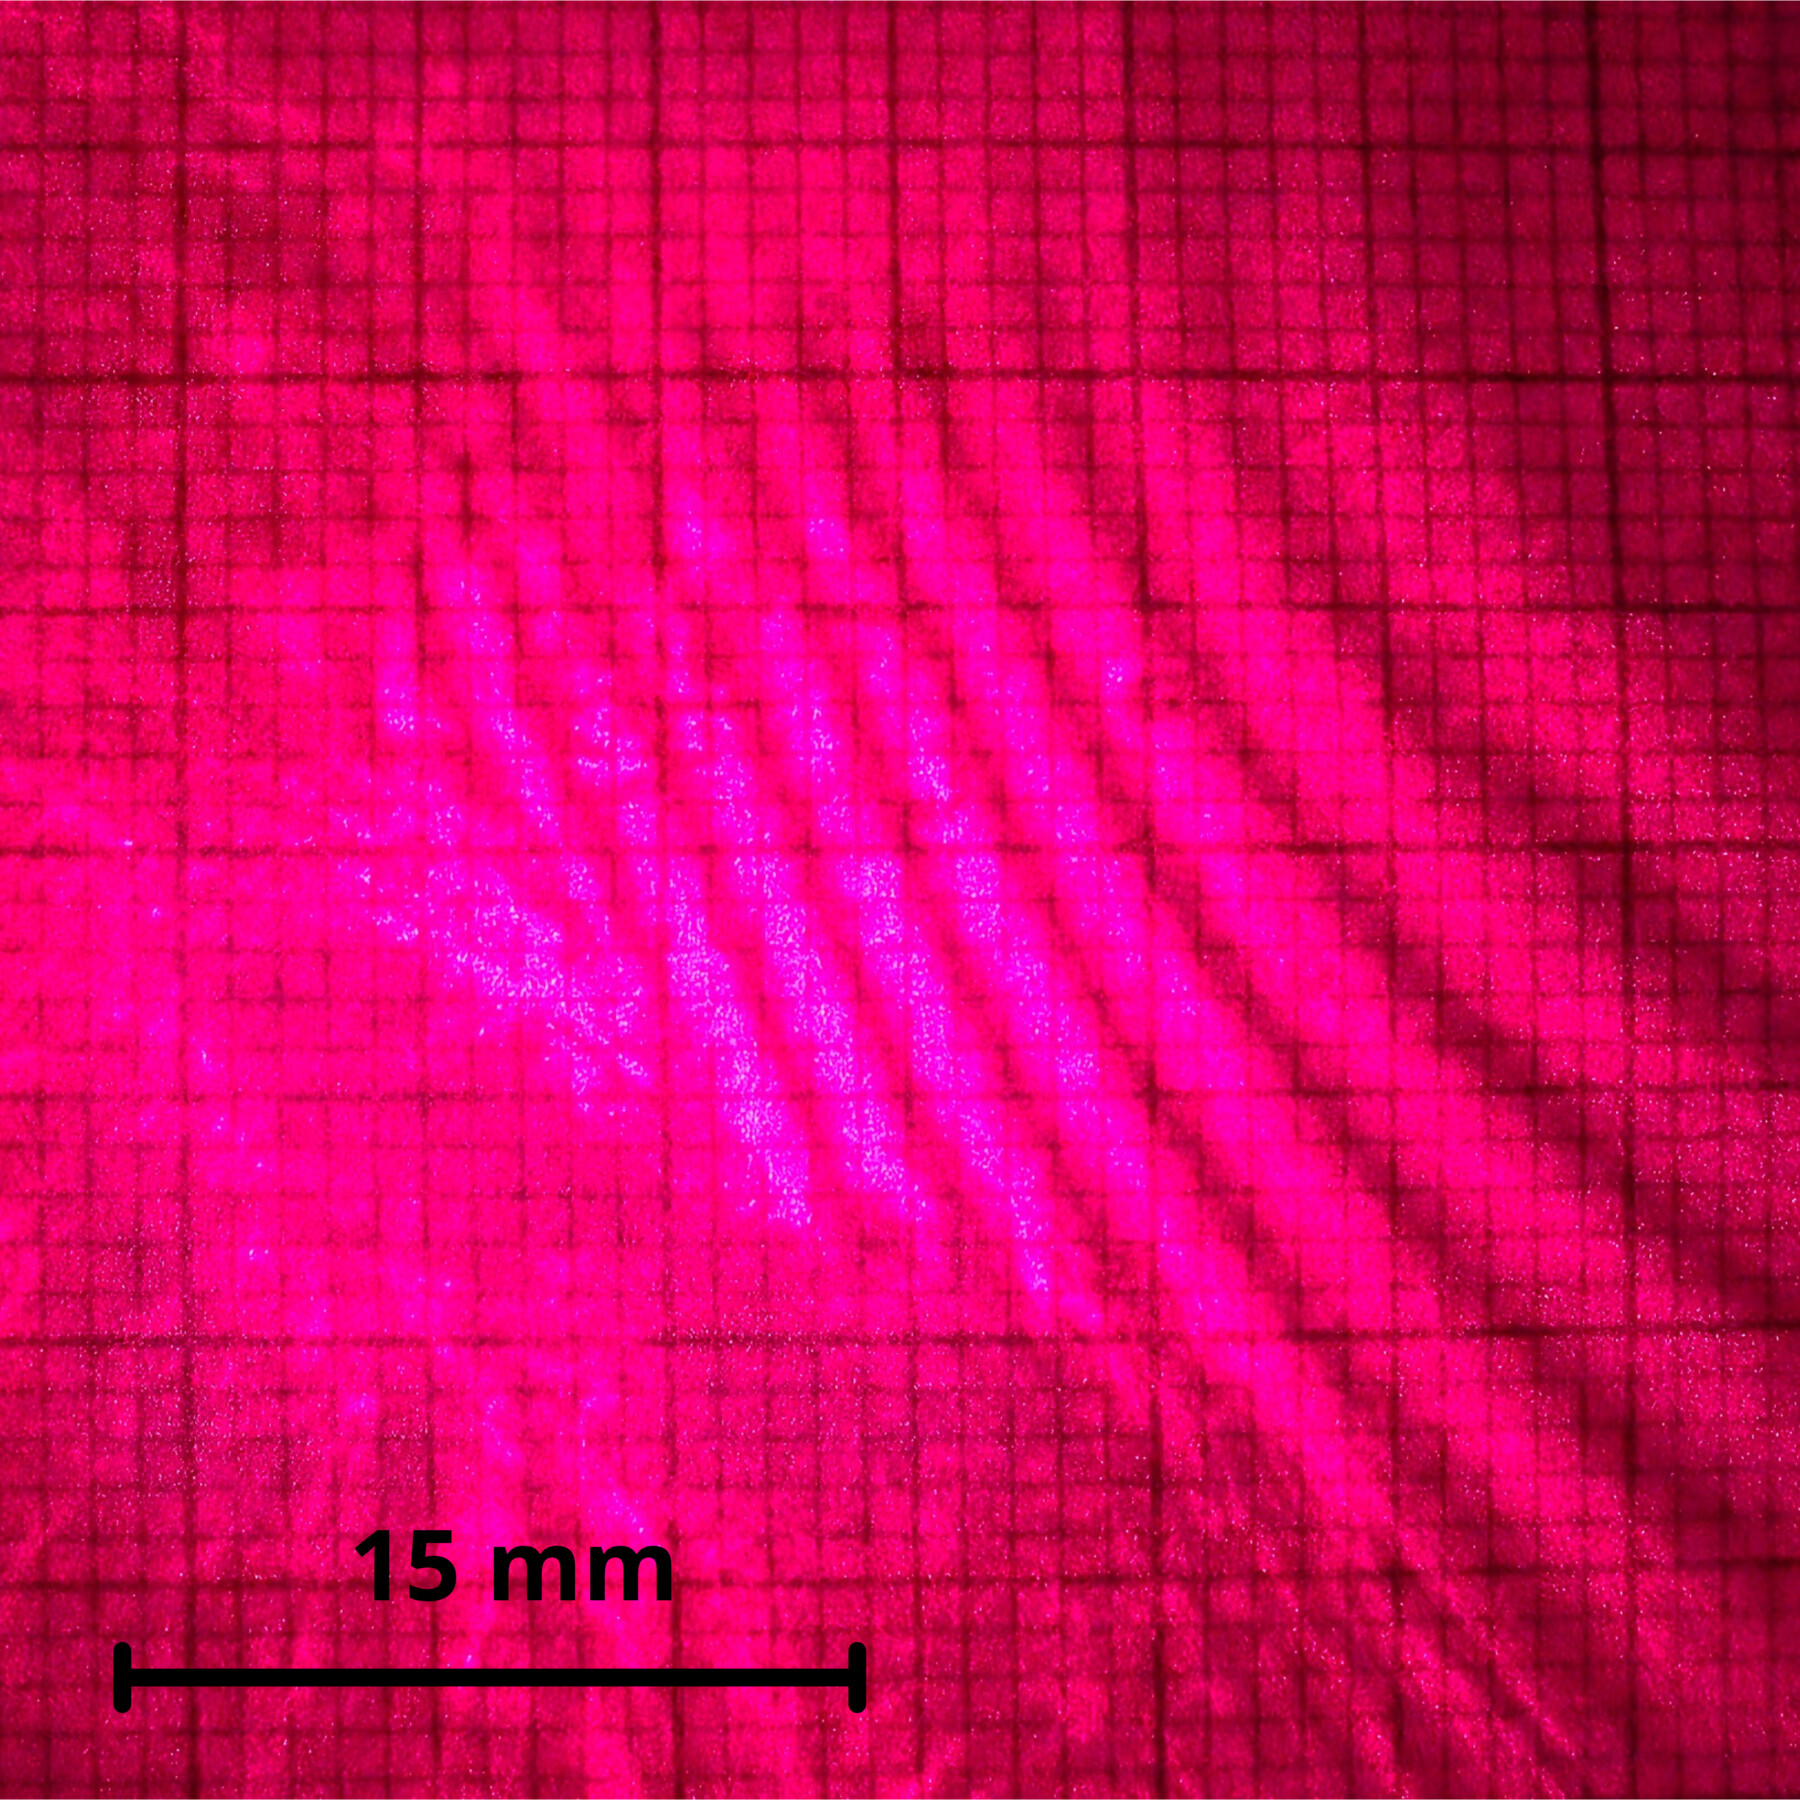
\includegraphics[width=\textwidth]{images/pattern_4mm_back_compressed.jpg}
        \caption{Pattern 4mm}
        \label{fig:pattern_2mm_back_b}
    \end{subfigure}
    \caption{Interference pattern obtained from the interferometer through a piece of paper as objective. a) Interferometer at 2 mm of the objective; b) Interferometer at 4 mm of the objective.}
    \label{fig:patterns_back}
\end{figure}



\Cref{fig:patterns_back} shows the experimental interference patterns projected onto a millimeter-ruled paper screen at screen distances of $2\text{ mm}$ and $4\text{ mm}$ from the interferometer output. In both configurations, at the center the fringes are approximate parallel to each other and at the borders start to catch on the characteristic curvature from Michelson interferometer fringes, this has to do with the alignment of the optical components and the lens positioning offset with respect to the optical axis.
